\documentclass[10pt,twoside,twocolumn,openany]{dndbook}
\let\chaptername\relax

\usepackage[spanish]{babel}
\usepackage[utf8]{inputenc}
\usepackage[singlelinecheck=false]{caption}
\usepackage{listings}
\usepackage{shortvrb}
\usepackage{stfloats}
\usepackage{ifoddpage}
\usepackage{graphicx}
\usepackage{tikz}
\usepackage{fontawesome5} % Paquete para íconos
\usepackage{cuted}
\usepackage{hyperref}

\hypersetup{
  colorlinks=true,
  linkcolor=black,  % Color de los enlaces internos (por ejemplo, dentro de la tabla de contenidos)
  urlcolor=magenta,   % Color de los enlaces a URLs
  %%citecolor=green,
  pdfauthor={Moisés Serrano Samudio},
  pdftitle={Luna de sangre},
  pdfsubject={one-shot},
  pdfkeywords={Dungeon and Dragons, DnD, 5e, secuestro, rescate}
}

\DndSetFonts[section-style = \linespread{.9} \color{titlered} \LARGE \scshape \RaggedRight]

\title{Luna de sangre\\
\large One shot para personajes de nivel inicial}
\author{linkmoises}
\date{\today}

\begin{document}

%%
%% Portada
%%
\newpage
\thispagestyle{empty}
\mbox{}
\begin{figure}
  \begin{tikzpicture}[remember picture,overlay]
    \begin{scope}
    \node [xshift=0cm,yshift=0cm] at (current page.center){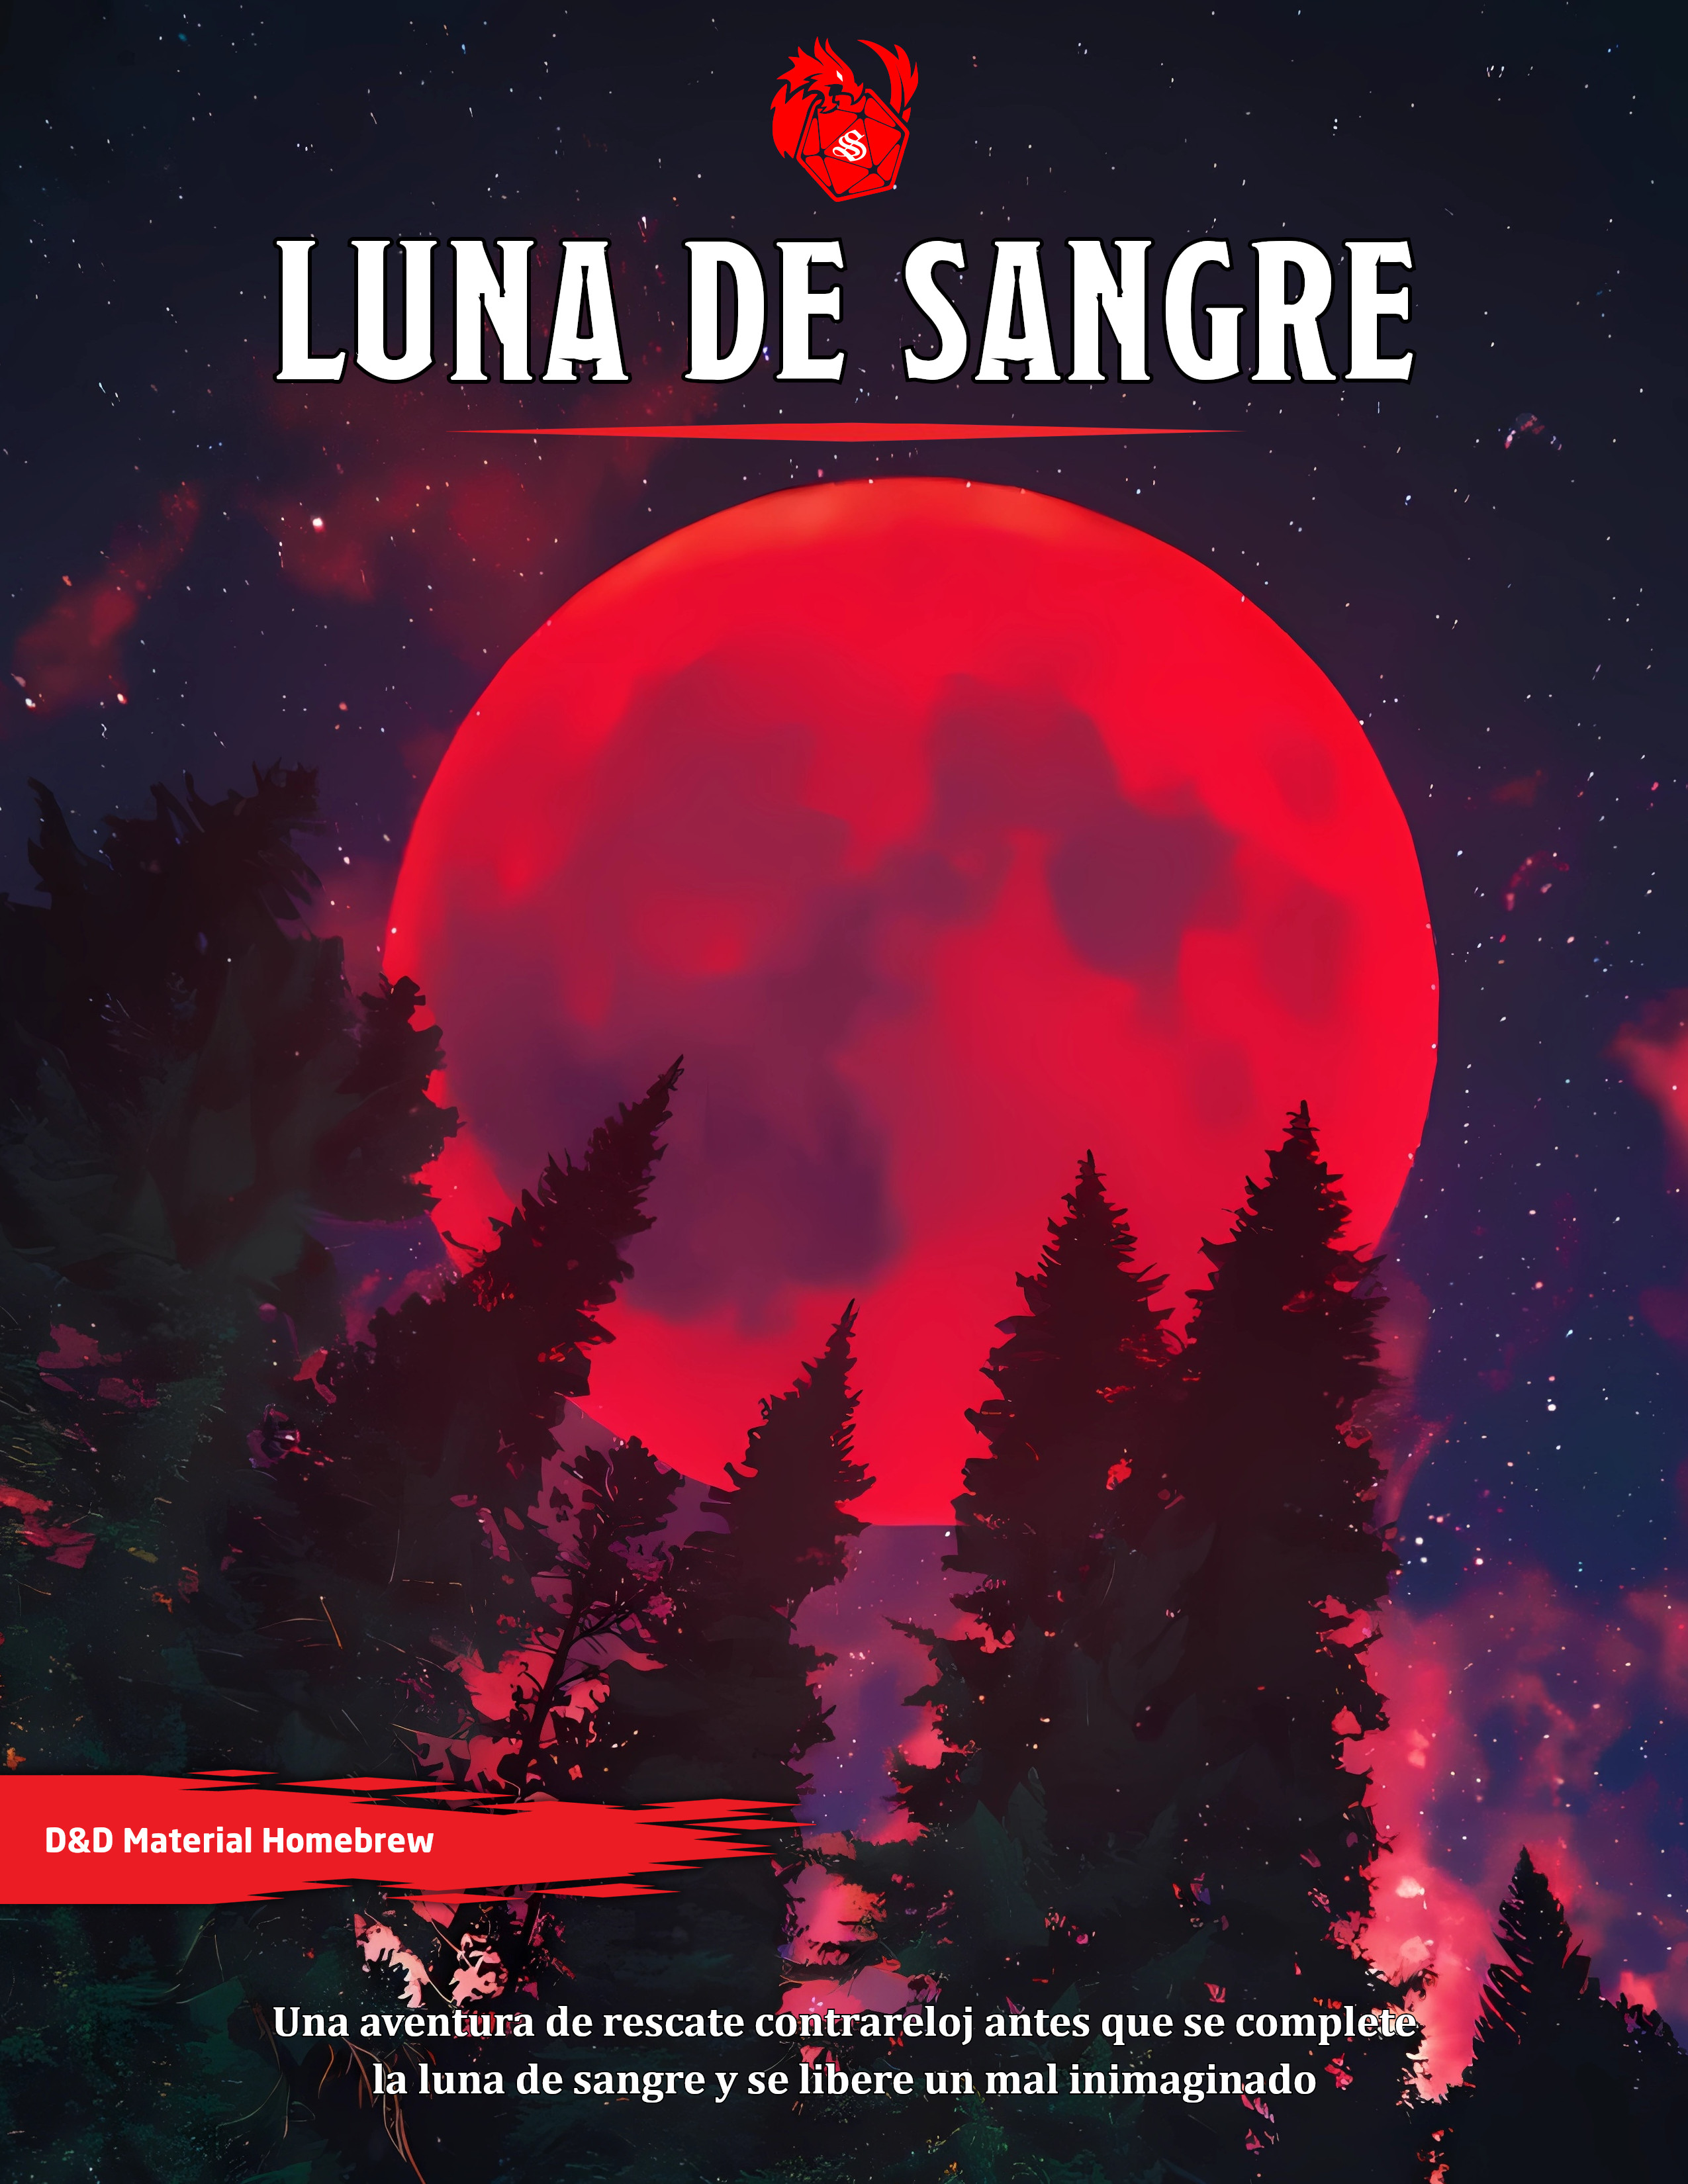
\includegraphics[width=\paperwidth]{covers/1-luna-de-sangre.jpg}};
    \end{scope}
  \end{tikzpicture}
\end{figure}
%%
%% Finaliza portada
%%

%%
%% hack para que texto de licencia se muestre en página siguiente
%%
\newpage
\thispagestyle{empty}
\mbox{}

%%
%% Página para licencia
%%
\newpage
\thispagestyle{empty} % Elimina el pie de página con numeración

\begin{center}
  \vspace*{\fill} % Ajustar espacio vertical antes del texto
  \begin{minipage}[b]{\textwidth}
      \justifying % Cambiar a justificado
      \noindent % Eliminar la sangría en la primera línea
      \faCreativeCommons \faCreativeCommonsBy \faCreativeCommonsNc \faCreativeCommonsSa \hspace{0.5em} 
      Contenido protegido por una \textbf{Licencia CC BY-NC-SA}
      \vspace{1em} % Espacio vertical entre título licencia y texto

      {\footnotesize
      \noindent
      El contenido escrito de este documento está protegido por la Licencia Creative Commons 
      Atribución-NoComercial-CompartirIgual 4.0 Internacional 
      \href{https://creativecommons.org/licenses/by-nc-sa/4.0/deed.es}{(CC BY-NC-SA)}. Esto 
      significa que puedes compartir, copiar, redistribuir, adaptar y crear a partir de este 
      contenido, siempre y cuando otorgues la debida atribución al autor original y compartas tus 
      derivados bajo una licencia similar que no permita el uso comercial. Esta obra incluye 
      materiales extraídos del 
      \href{https://dnd.wizards.com/es/resources/systems-reference-document}{Documento de 
      referencia del sistema 5.1 (“SRD 5.1”)} de Wizards of the Coast LLC. El SRD 5.1 tiene la 
      licencia \href{https://creativecommons.org/licenses/by/4.0/legalcode.es}
      {Creative Commons Atribución/Reconocimiento 4.0 Licencia Pública Internacional}. 
      Las imágenes e ilustraciones incluidas en este documento son creaciones de sus respectivos 
      autores y están protegidas por sus propias licencias. Consulta la sección créditos para 
      obtener información sobre las licencias individuales y conocer el trabajo de sus autores.      
      }
    \end{minipage}
\end{center}

\frontmatter

\maketitle

\tableofcontents

\mainmatter

\part*{Luna de Sangre}

%%
%% Página para Sesión Cero
%%
\chapter*{Sesión Cero}
\addcontentsline{toc}{chapter}{Sesión Cero}

\begin{tikzpicture}[remember picture, overlay]
  \node [xshift=0cm,yshift=-7cm] at (current page.north) {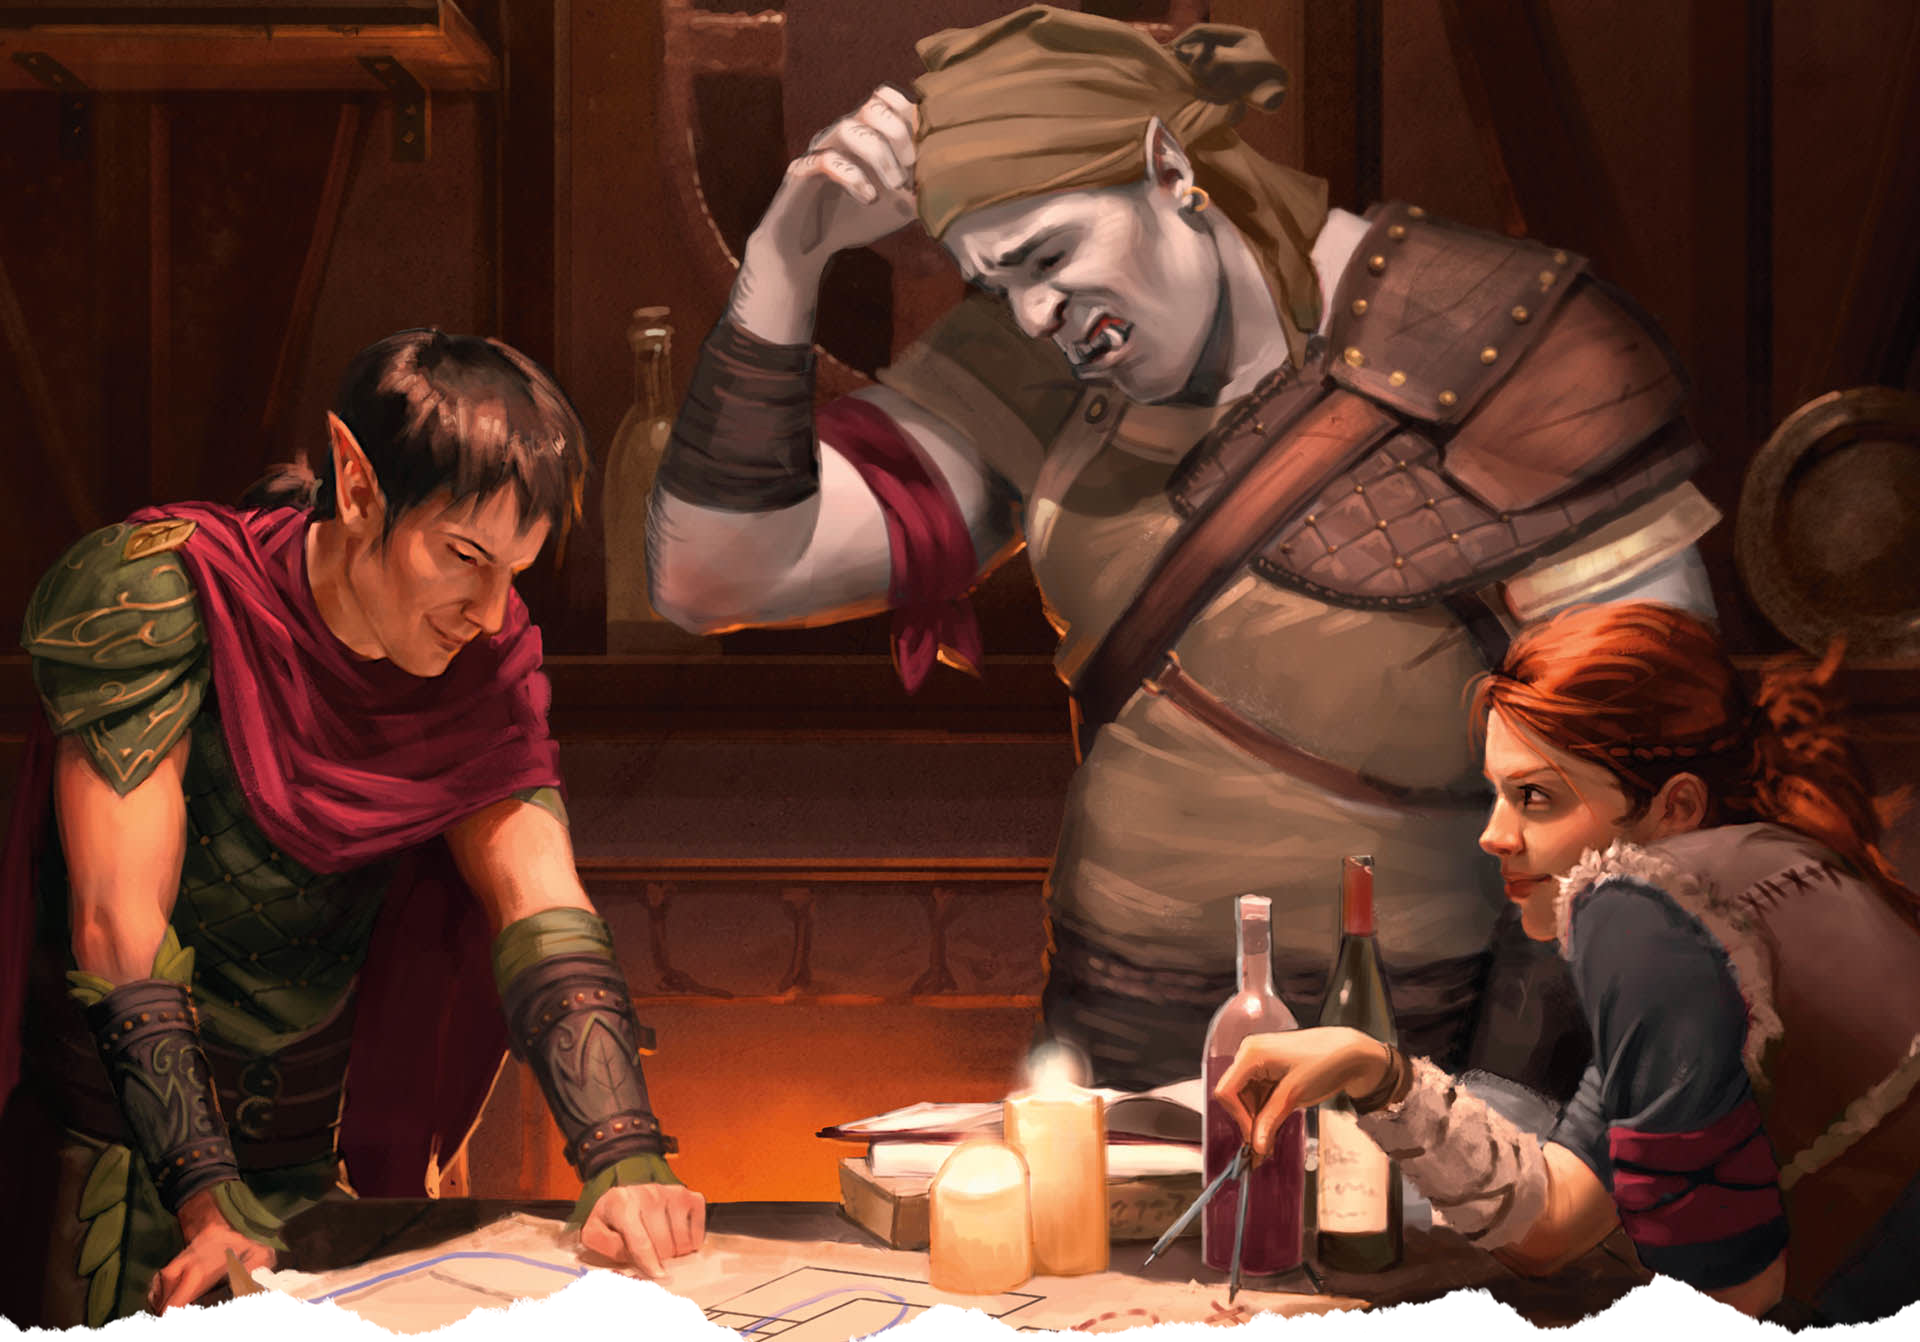
\includegraphics[width=\paperwidth]{media/zero.png}};
\end{tikzpicture}

%% Este bloque introduce un png transparente que empuja el texto a dos columnas hacia abajo
\begin{strip}
  \centering
  
\includegraphics[width=\textwidth]{media/invisible.png}
\end{strip}
%%

\DndDropCapLine{L}{a sesión cero} es una excelente manera de asegurarse de que un one-shot o 
campaña comience y finalice sin problemas. Lo primero que hay que recordar es que el juego incluye 
a los jugadores en la mesa y también al director del juego o Dungeon Master (DM). El objetivo es 
que todos se diviertan y se establezcan expectativas claras para para beneficio de todo el grupo. 
Aún en los one-shots que son sesiones cortas resulta buena idea invertir al menos unos 15-30 
minutos antes de iniciar para dejar todo claro.

\section*{Una nota para el DM}

\begin{DndReadAloud}
  En la preparación de la batalla siempre he comprobado que los planes son inútiles, pero la 
  planificación es indispensable. \\
  \emph{Dwight D. Eisenhower}
\end{DndReadAloud}

Esta cita es un amable recordatorio de que a veces toda la planificación puede irse al traste 
en un juego de rol por las decisiones de los jugadores. A veces hay que ser flexibles o improvisar 
sobre la marcha.

Este one-shot fue creado como una aventura introductoria rápida para jugadores noveles que se integran 
a nuestra mesa en Arcanos del Norte y para uso con una hoja de personaje simplificada, aunque 
también se puede emplear la oficial. Incluimos al final ganchos a las aventuras oficiales de las 
cajas de inicio de Dungeons and Dragons.

\section*{Consejos para jugadores}

La información plasmada aquí está dirigida mayormente a los jugadores y sobre todo a mantener la 
sesión balanceada y que transcurra sin obstáculos. Estos son algunos consejos:

\begin{itemize}
  \item \emph{Minimizar distracciones}. Esto tiene que ver sobre todo con el uso de teléfonos 
  móviles, ten en cuenta que si te distraes te perderás la diversión.
  \item \emph{Mantener los personajes simples}. Esta aventura no requiere personajes tan complejos.
  Si tienes un personaje de una clase lanzadora de hechizos con algunos cantrips y unos 3 ó 4 
  hechizos de nivel 1 será suficiente. A medida que ganes experiencia en el juego y manejo de tu 
  personaje podrás añadir mecánicas más complejas.
  \item \emph{Intermezzo}. La aventura está dividida en 2 partes, se puede realizar un intermezzo 
  al final de la primera parte para algunos snacks, ir al baño, etc.
\end{itemize}

\section*{Descripción breve}

Faltan 1 día para un evento astronómico de suma importancia arcana en Faerûn, la \textbf{Luna de Sangre}. 
Durante siglos diversas razas han realizado rituales para pedir favores a sus deidades. Durante 
estos eventos, los límites entre los planos se debilitan y es fácil pasar de un plano a otro.

Esta aventura titulada Luna de Sangre es un one shot. Transcurre en aldeas cercanas a Phandalin en 
la región de la Costa De La Espada en Faerûn. Trata sobre el secuestro de unas niñas y un 
sacrificio ritual. Predominan en esta aventura el combate y la exploración.

\section*{Duración}

Se estima que esta aventura puede ser completada en una sola sesión con una duración de 60 a 90 
minutos.

\section*{Reglas de casa}

Las reglas de casa son reglas que no están escritas en los manuales oficiales de Dungeons and 
Dragons, pero que consideramos pueden ayudar a que las acciones en la mesa y la fluidez del juego 
sean mejoradas.

\begin{itemize}
  \item Las pociones curativas se pueden usar como una acción adicional en tu turno, sin la 
  penalización descrita en el manual del jugador como acción del turno. Los mismo aplica para 
  hechizos de curación, excepto que se cure a otra persona entonces sería una acción.
  \item Si recibes un token de inspiración por parte del DM. Esta representa una tirada de 
  ventaja que puedes usar en el momento que desees.
  \item En tiradas de iniciativa, un 20 natural permite elegir al jugador su orden de 
  iniciativa luego de establecidas todas las iniciativas.
  \item Una alternativa en las tiradas de iniciativa, puede ser que el mismo grupo de jugadores
  se organice tácticamente en los ataques. Podría ser que el grupo quiera que el bárbaro inicie
  el ataque y los lanzadores de conjuros finalicen la ronda.
  \item En tiradas de ataque, un 20 natural dobla el máximo del dado de golpe y su bonificador 
  de competencia.
  \item Si una criatura o personaje sufre daño por caída que excede su puntuación de Constitución, 
  sus puntos de vida caen a 0 y queda inconsciente. Si una criatura o personaje sufre un daño por 
  caída que excede el doble de su puntuación de Constitución, muere instantáneamente.
\end{itemize}

\section*{Reglas de creación de personajes}

Es conveniente que los personajes traigan sus personajes ya creados para no prolongar la sesión. 
Se admiten todas las clases ya publicadas en los libros oficiales de Dungeons and Dragons: Manual 
del jugador, Guía de Xanathar para todo, El Caldero de Tasha para todo. El inventario de cada 
personaje y hechizos disponibles se pueden elegir de entre estas opciones.

\section*{Herramientas de seguridad}

Las herramientas de seguridad están diseñadas para que el juego sea divertido para todos los 
jugadores, incluido el DM. Establecer expectativas con todos en la mesa antes de jugar, puede 
ayudar a garantizar que todos estén cómodos, seguros y no se sorprendan más adelante en el juego. 
En esta hoja, hemos incorporado dos técnicas llamadas líneas y velos que ayudarán al DM y los 
jugadores a manejar determinadas situaciones para que todos se diviertan.

\subsection*{Líneas}

Las líneas son límites estrictos sobre temas o eventos con los que el director del juego o los 
jugadores no se sienten cómodos participando. Estos temas o eventos son "líneas" que no se pueden 
cruzar durante todo el juego. Estos temas nunca deberían usarse en un juego ni aludirse en absoluto.

Se consideran líneas: violencia sexual, abuso infantil, torturas muy descriptivas. Si en el grupo 
alguna persona presenta una fobia, es recomendable incluirla dentro de las líneas.

\subsection*{Velos}

Los velos son límites suaves sobre temas o eventos que solo se describirán con detalles limitados 
y/o solo sucederán detrás de escena. Estos pueden incluir temas que los jugadores en la mesa están 
de acuerdo con que sucedan, pero que solo se describen con detalle limitado. Estos pueden incluir 
temas sexuales y sangre extrema que se supone que sucede y se describe a través de un montaje 
rápido o solo unas pocas palabras que digan que sucedió con poco detalle.


%%
%% Aquí en adelante inicia la aventura
%%
\chapter*{Luna de Sangre}
\addcontentsline{toc}{chapter}{Luna de Sangre}

\DndDropCapLine{L}{as niñas de aldeas cerca de Phandalin} han estado desapareciendo en los 
últimos 3 días. Nadie sabe que está ocurriendo, solo se sabe que se acuestan y a la mañana 
siguiente ya no están. Los padres y madres preocupados ahora duermen en la misma habitación de
sus hijos o les amarran a la cama al momento de dormir para evitar que desaparezcan. La última 
niña en desaparecer fue la hija del gobernador hace solo unas horas. Han desaparecido un total de 
12 niñas en ese lapso de tiempo.

Desde entonces, el gobernador, Tormund Esses, ha colgado carteles por toda la aldea y en Phandalin 
ofreciendo recompensas por quién pueda dar información sobre el paradero de las niñas o las pueda 
encontrar.

\section{Presentación y gancho de aventura}

Los aventureros son aprendices de héroes que intentan ganar algo de fama y dinero. Varios aventureros 
se presentaron el último día para enfrentar el reto y encontrar a los niños. Por desgracia, ya sea 
por mala suerte o inexperiencia, hasta ahora no se sabe de ninguno de ellos.

Dependiendo de la conformación del grupo o del tiempo de disponible, la aventura puede ser abordada
permitiendo que el grupo explore las aldeas cercanas y que encuentren un rastro que se interne al 
bosque cercano. Luego de esto, se encuentran con Fred. Fred, es un chico de 15 años. Fue testigo 
del rapto de una de las niñas e intento seguir a los goblins que la llevaban, pero se perdió en 
el camino.

\begin{DndComment}{Búsqueda}
  Los jugadores al interrogar a Fred podrán obtener la siguiente información:

  \begin{itemize}
    \item Se llama Fred...
    \item Alcanzó a ver unos hombres pequeños cargando a una niña dormida hacia el bosque
    \item Intento seguir el rastro...
    \item Se perdió en el camino
    \item Desea acompañar al grupo en la búsqueda, pues una de las niñas es hermana de él
  \end{itemize}
  
\end{DndComment}

Una vez el grupo comience a buscar el rastro dadas las indicaciones de Fred, activarán una trampa
oculta en el camino. Queda a discreción del DM decidir cómo fueron capturados los jugadores y
Fred y en qué momento. En todo caso, los miembros del grupo llegan inconscientes a las celdas 
dónde los tienen prisioneros en el Campamento Goblin.

Los aventureros despertarán cerca de las diez de la noche, en celdas a la intemperie hechas por vigas de 
madera, algunos barrotes de hierro y sin ninguna de sus armas.


\section{Parte 1: Campamento Goblin}

A pesar de preferir ambientes oscuros y húmedos como cuevas, por alguna razón diferente a la usual 
un grupo de poco más de 20 goblins (Manual de Monstruos, pág.: xxx) han establecido un campamento 
en las profundidades del bosque rodeado de árboles altos al lado de un río. 

Hay 5 tiendas improvisadas con una principal del doble de tamaño que las otras. La explanada del 
campamento ofrece un terreno bastante llano. Frente al campamento central, hay un pozo que ha sido 
excavado de manera circular rodeado por piedras con marcas rúnicas. Frente al foso, hay una mesa 
dispuesta como altar ceremonial.

Las celdas están ubicadas al sur del campamento y en su mayoría tienen 3 niñas por cada celda. Hay 
niñas asustadas en su mayoría, agotadas por la mala alimentación y deshidratadas algunas por qué 
están presentando vómitos y diarrea.

En la figura \ref{fig:camp1} se puede apreciar la disposición general del campamento goblin.

\begin{figure*}[hb!]
  \centering
  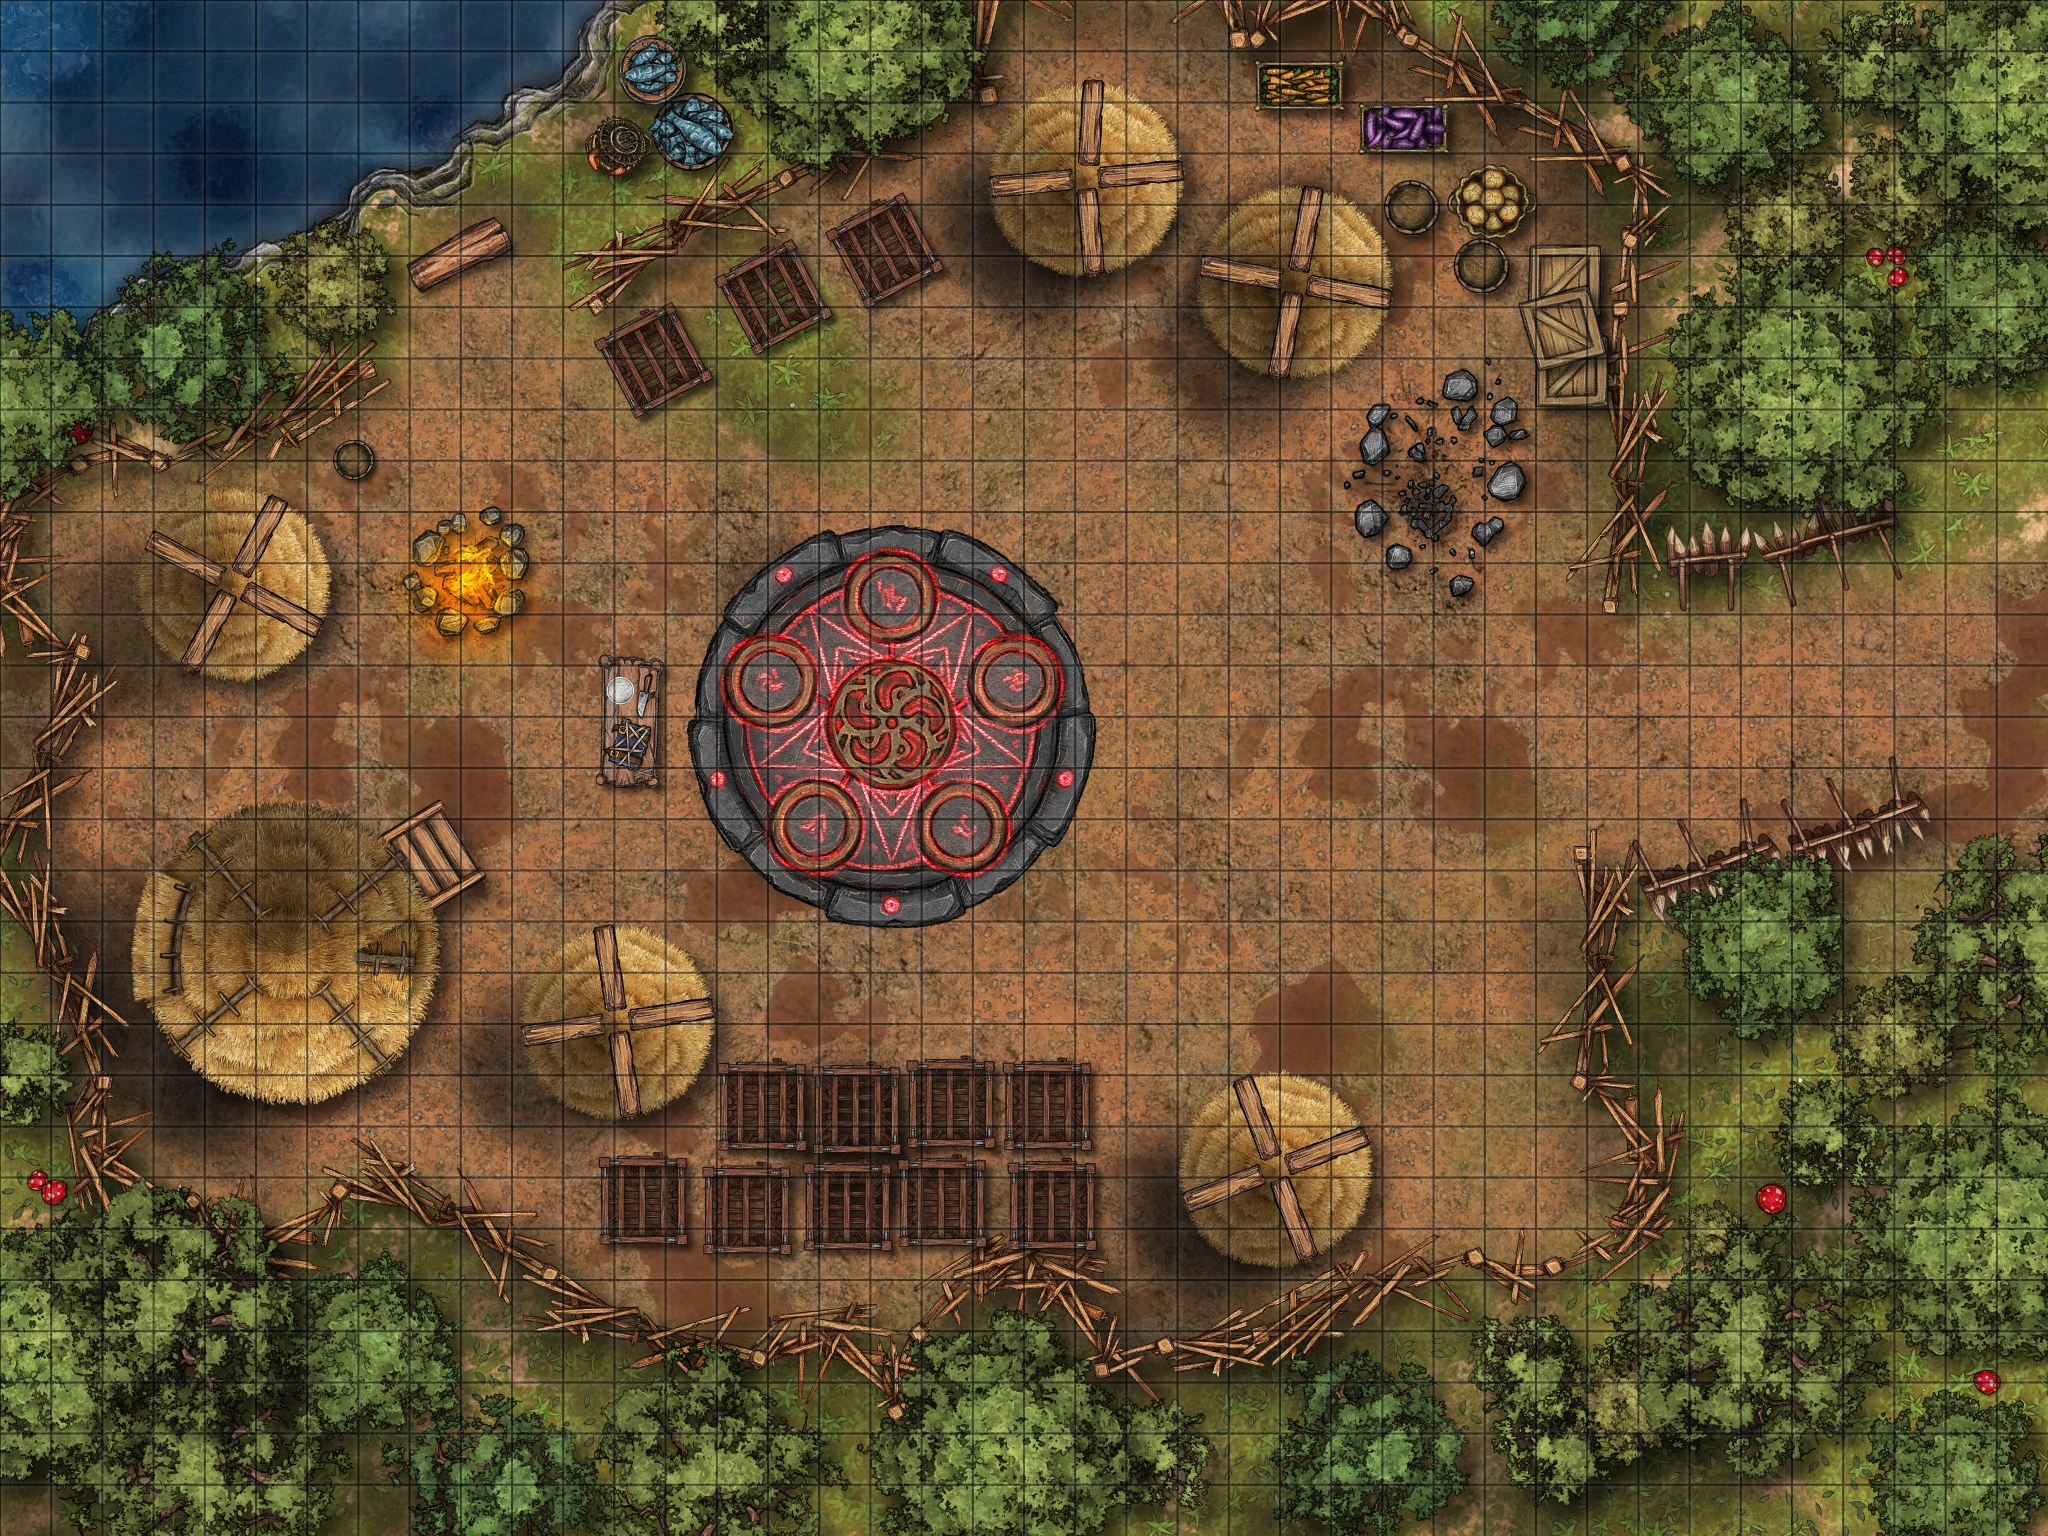
\includegraphics[width=\textwidth]{maps/goblin-camp.jpg}
  \caption{Campamento Goblin}
  \label{fig:camp1}
\end{figure*}

\begin{DndComment}{Prisioneros}
Los jugadores estarán repartidos de manera individual en cada celda. Cuando empiecen a preguntar qué 
ha pasado o donde están, podrán conseguir la siguiente información de un prisionero (perteneciente 
a una de las aldea) que llegó el día anterior al grupo, llamado Fred.

  \begin{itemize}
    \item Todas las niñas desaparecidas están repartidos en las celdas y tienen 12 años.
    \item Los miembros del clan se escabullen en la noche y secuestran niños y niñas en sus casas en las aldeas cercanas.
    \item Un goblin grande encapuchado con la piel de color naranja dirige a los goblins. Su nombre es Grommash Tejesombras y dirige a los goblins con mano de hierro manteniéndolos aterrorizados.
    \item Grommash tiene una mascota, Sombrafauces, un perro del inframundo de tres cabezas, que alimenta con carne humana (y también de goblins). El chamán hobgoblin lo usa para intimidar a los goblins y a los prisioneros.
    \item Grommash se la pasa hablando de una luna de sangre.
  \end{itemize}

\end{DndComment}

\DndArea{Tienda principal}
Se encuentra en el centro del campamento, es más grande y ornamentada que las otras, tiene una sola 
entrada y salida. Es custodiada siempre por dos goblins. En su interior, el piso es de piel de oso pardo 
y con una silla de madera tallada a manera de trono. Hay varios alijos de madera y un arcón de hierro 
dónde el clan guarda sus tesoros robados más importantes. Llama la atención una jaula de acero 
inmediatamente a la derecha luego de la entrada, dónde se encuentra Sombrafauces. Las paredes están 
cubiertas de pieles y trofeos de batalla. En el interior, los jugadores pueden encontrar un mapa 
detallado de la región, marcando algunos lugares de interés.

Si alguno de los jugadores tiene la iniciativa de dar una hojeada al mapa, se dará cuenta que 
muestra el área cercana al bosque donde se encuentran. Verán un total de 12 cruces marcadas en el 
mapa en color rojo y otras 5 cruces en azul distribuidas en el terreno del bosque. En una prueba 
exitosa de \textbf{investigación (Inteligencia) CD 15} deducirán que las cruces rojas son las 
ubicaciones donde fueron secuestradas las niñas. En una prueba exitosa de 
\textbf{investigación (Inteligencia) CD 20} deducirán que las cruces azules están ubicadas en 
las posibles rutas de escape del campamento.

También en esta área los jugadores encontrarán sus armas que les fueron quitadas al momento de ser
emboscados al inicio de la aventura, amontonadas en una esquina.

\DndArea{Pozo de sacrificios}
Esta área es un círculo excavado en el suelo, rodeado de piedras y adornado con runas oscuras. En esta 
área Grommash realiza sus rituales de sacrificio. Frente al pozo, los jugadores pueden encontrar 
una mesa ritual sobre la que hay un cuenco ritual, un cuchillo y un libro ritual.

\DndArea{Tiendas goblins}
Las tiendas improvisadas de los goblins son pequeñas y sucias, con literas apiladas en desorden. Hay 
varios catres de cuero, una mesa de madera improvisada donde colocan su equipo y varios barriles. 
Algunos goblins guardan pequeños tesoros personales en sus literas, como monedas de oro o joyas robadas.

En una de las literas, los jugadores pueden encontrar una carta escrita en un idioma desconocido 
(a menos que algunos de los jugadores tenga competencia en idioma ghukliak) que 
puede revelar información sobre los planes de Grommash. En una prueba exitosa de 
\textbf{investigación (Inteligencia) CD 20} podrán deducir por los dibujos que se trata de 
trampas. Si alguno de los jugadores supero con éxito la prueba de las cruces azules en la tienda 
principal relacionará las informaciones y con una prueba exitosa de 
\textbf{investigación (Inteligencia) CD 10} podrá deducir que las trampas están ubicadas en las
rutas de escape del campamento.

Cerca al río hay tres jaulas vacías con cadenas en su interior. Son usadas para amarrar a los 
huargos que montan los goblins que patrullan alrededor del campamento.

\DndArea{Área de celdas}
Este lugar está rodeado por una empalizada de madera y alambre de púas. En el suelo de tierra, hay 
varias celdas rudimentarias, cada una con barrotes de hierro. 

\section{Eventos}
A medida que evoluciona la aventura, ocurrirán una serie de eventos que motivarán a los jugadores a 
tomar desiciones. Como evolucione la partida dependerá en gran parte de como los jugadores reaccionen 
luego de los dos eventos principales.

\begin{DndReadAloud}
  A medida que avanza la noche, los prisioneros caen en cuentra de la situación desesperada en la que 
  se encuentran. Grommash, el chamán hobgoblin se acerca a las improvisadas celdas diciendo en lengua 
  común, aún falta para la luna de sangre, pero tengo ganas de divertirme. Los mira a todos... 
  uno por uno, con una mirada que despierta un miedo interior que no habían sentido antes. Las niñas 
  se agitan en sus celdas. Luego a los pocos segundos se levanta su mano derecha con un índice acusador...
\end{DndReadAloud}

En este momento ha elegido a Fred. Fred, es un chico de 15 años. Fue testigo del rapto de una de las 
niñas, pero al seguir a los goblins que la llevaban, activó una de las trampas en el camino provocando 
así su propia captura.

\begin{DndReadAloud}
Los goblins sacan a Fred de su celda y lo llevan ante su jefe. Grommash le dice en lengua común, eres 
libre de irte muchacho. Tu vida no me interesa. Raudo y veloz, presa del miedo echa a correr hacia el 
oeste por el camino que lo habían traido. Cuando casi llegaba al límite del campamento con el bosque, 
Grommash dice "pero Sombrafauces no ha comido el día de hoy, a por él". Un aullido infernal retumbo 
en los oídos de los prisioneros y ven con horror como una sombra infernal como un perro de dos cabezas 
hace carrera detrás de Fred. Cuando ya se hubo internado en el bosque, unos segundos después escuchan 
gritos y luego silencio. Tras unos eternos minutos, emerge de las sombras, Sombrafauces. Lleno de sangre 
marcha hasta donde se encuentra su amo. Grommash dice en lengua común, aquellos que osen escapar 
sabrán a que atenerse.
\end{DndReadAloud}

La noche de la luna de sangre, Grommash empezará un ritual en el foso de sacrificios desde el inicio de la 
luna de sangre a las 11 de la noche. A partir de esta hora conducirá las niñas custodiadas por los 
goblins hacia el foso de los sacrificios. Grommash controlará telepáticamente, con ayuda de un 
amuleto que cuelga de su cuello con símbolos que dan cuenta que se trata de un objeto infernal, 
a una por una haciendo que se corte el cuello frente al altar improvisado y el foso de sacrificios. 
Una chica cada cinco minutos, mientras colecta la sangre que mana del cuello de sus víctimas en el 
cuenco ritual. Cuando la chica en cuestión comience a agonizar de pie, sus goblins la arrojarán al 
foso de sacrificios.

Que ocurra o no este último evento estará determinado por las acciones de los personajes jugadores.

\section{Fuga}

Hay que destacar que si los jugadores intentan escapar a lo loco, confrontando directamente a los 
enemigos, lo más seguro es que acaben muertos. Los adversarios poseen una abundante ventaja numérica y 
podrían poner en un serio aprieto a los jugadores si optan por una estrategia directa.

Antes de iniciar el ritual, Grommash se encontrará en la tienda principal realizando algunos
rezos a sus deidades demoníacas preparandose para la luna de sangre.

Esta aventura está preparada para que los jugadores planeen su fuga y la del resto de las niñas prisioneras. 
Estos pueden intentar encargarse de algunos de los goblins, pero lo más seguro es que alguno muera por 
el camino si hay combates abiertos. Lo mejor será que los jugadores intenten acabar con los enemigos 
poco a poco, mediante subterfugios, intentando escapar de sus celdas y acabando con los goblins en 
pequeños grupos mientras descansan en sus tiendas.

Si alguno de los jugadores pertence a la clase pícaro o es competente con herramientas de ladrón 
y supera con éxito una prueba de característica \textbf{destreza CD 10} podrá abrir la cerradura
sin mayor deficultad estando dentro de la celda, de lo contrario la CD a superar sera 15. Una vez 
fuera, podrá abrir con éxito todas las cerraduras 

Cada uno de los personajes que logre salir de su celda, tendrá que realizar una prueba de 
característica \textbf{sigilo (destreza) CD 10} para evitar ser detectado por los goblins que 
custodian las celdas.

Otra opción para el grupo sería interactuar con Grommash y tratar de convencerlo para que de forma 
pacífica libere a las niñas. Sin embargo, esta opción sería poco viable dado el alineamiento 
caótico malvado.

Los eventos de combate están pensados para que, de tener éxito, los jugadores se enfrenten poco a poco 
a todos los enemigos en cantidades asumibles, aunque podrían sufrir el desgaste, sobre todo de cara al 
último enfrentamiento.

Los jugadores superarán esta parte de la aventura si todos los miembros del campamento se han rendido 
o han sido muertos. Cómo recompensa obtendrán un item mágico del alijo de Grommash y recuperarán sus 
armas y armaduras básicas.


\section{Parte 2: Huida a la aldea}

Los jugadores deben escapar con las niñas del campamento y llevarlas sanas y salvas hasta la aldea. 
Antes de ello deberán sortear una serie de trampas que han dispuesto los goblins en el camino de salida. 
El campamento se halla unos 5 millas bosque adentro, en un terreno sumamente accidentado y que 
permanentemente esta cubierto de una niebla espesa. Con el escape ocurriendo durante la noche 
la temperatura fría del ambiente, condiciones de niebla densa y la luna de sangre ocurriendo dando 
un tono rojizo al ambiente, la visión estará limitada a unos 30 pies de distancia. La salida se 
encuentra al oeste del campamento. Si intentan escapar por el río, una de la niñas dirá que eso 
las alejará de la aldea porque es un camino más largo.

\begin{DndReadAloud}
Mientras escapan hacia la aldea, cuando ya se han alejado unos 300 pies del campamento, escuchan 
un aullido gutural. Una brisa gélida, suave y ominosa se encuentra con los jugadores. La oscuridad
se cierra totalmente ante el grupo y el tono rojo que hay en el ambiente desaparece por un momento.
La tierra tiembla por un momento.
\end{DndReadAloud}

Unos goblins patrullan alrededor del campamento a unos 100 pies montados sobre huargos (Manual 
de Monstruos, pág.: xxx). Uno de ellos se da cuenta de la huida y su huargo lanza un aullido 
alertando a otros.

Habrán 3 trampas dispuestas en el camino. La primera un foso cubierto por una enramada a 30 pies de e
la salida. Es posible que caigan si no superan una prueba de Sabiduría (percepción) superior a 15.

La segunda trampa es un sistema que lanza dardos qué están impregnados con un somnifero en sus puntas. 
Si alguno del grupo es alcanzado, ralentizara el avance como grupo, al obligar a cargar a los afectados 
y predisponiéndolos a ser alcanzados por los goblins montados en huargos y obligando al grupo a 
enfrentarlos.

Una tercera y última trampa estara esperándolos a 500 pies de la aldea. Se trata de otro foso cubierto
por una enramada y que es custodiado de manera oculta por 4 goblins arqueros del campamento desde los 
árboles esperando por cualquier incursión desde la aldea. 

Al llegar a la última trampa, son alcanzados por Grommash quien va montado sobre Sombrafauces.
Sombrafauces ha crecido en tamaño dos veces de la última vez que lo vieron. Grommash se ha desplazado
utilizando Teletransportación sombría. Grommash tiene un aura oscura y una mirada que recuerda las llamas 
infernales. Al realizar el ritual de luna de sangre ganó una acción legendaria.

\section{Conclusión}

Los jugadores superarán esta parte de la aventura si logran llegar a la aldea con las niñas. Si 
logran llegar con las 12 niñas recibirán una recompensa de 100 piezas de oro para todo el grupo. Si
muere alguna de las niñas recibirán una recompensa de 50 piezas de oro para todo el grupo.

Este es un buen momento para anunciar que los jugadores suben de nivel con todas las mejoras 
estadísticas que ello implica y el acceso a conjuros del siguiente nivel. Se otorgan 300 puntos 
de experiencia a cada jugador, los necesarios para alcanzar el nivel 2. Con esto estarán mejor 
preparados para una de las siguientes aventuras. Para subir de nivel seguir la recomendaciones
descritas en el Manual del Jugador.

\section{Epílogo}

Esta aventura corta sirve como introducción a Dungeons and Dragons y para conectar con las 
aventuras de la caja de inicio.

En medio de la celebración del pueblo por el rescate de las niñas, un par de NPCs estará conversando
lo suficientemente cerca del grupo una de estas dos opciones:

\begin{itemize}
  \item Si deseas conectar la Aventura de la \emph{Mina Perdida de Phandelver}: escucharán dos 
  enanos conversando sobre Gundren Buscarocas y el rumor de haber encontrado una enorme mina de 
  oro.
\end{itemize}

\begin{DndReadAloud}
  \textbf{Tornir}: ¡Hola Dalren! ¿Cómo has estado? Ha pasado tiempo... \\
  \textbf{Dalren}: ¡Tornir! ¡Hermano! ¿Cómo ha estado tu viaje a Waterdeep? \\
  \textbf{Tornir}: Pues fíjate que ha ido perfecto todo, logré llevar las armas en las que estaba 
  trabajando y venderlas. \\
  \textbf{Dalren}: ¡Qué bueno! ¿Y como ha estado nuestro primo, Gundren? \\
  \textbf{Tornir}: Pues fíjate que lo único que he escuchado sobre él es que encontró una mina 
  en la región de Phandelver \\
  \textbf{Dalren}: ¿Phandelver? se ha ido un poco lejos... He escuchado son terrenos inhóspitos
  para enanos... \\
  \textbf{Tornir}: Si, pero Gundren siempre ha sido así, le gusta la aventura... De hecho ayer 
  que pase por Phandalin escuché que está buscando unos escoltas para un cargamento. \\
  \textbf{Dalren}: ¡Je! Pero si aquí tienes al grupo que salvo a unas niñas que habían sido 
  secuestradas. \\
  \textbf{Tornir}: ¿Por eso es la fiesta? Y yo que pensé que era mi bienvenida... ¡Jajajajaja! les 
  comentaré. ¡Cuídate Dalren, ha sido un gusto verte! \\
  \textbf{Dalren}: ¡Tu también hermano! \\
\end{DndReadAloud}

Luego de esto, Tornir le comentará a alguno de los miembros del grupo sobre la solicitud de 
su primo Gundren.

\begin{itemize}
  \item Si deseas conectar la Aventura del \emph{Dragón del Pico Agujahelada}: esucharán a dos 
  jóvenes hablando sobre el rumor de avistamiento de una bestia cerca de las montañas.
\end{itemize} 

\begin{DndReadAloud}
  \textbf{Korey}: ¡Hola Robert! ¿Y esta fiesta? \\
  \textbf{Robert}: Es por unas niñas que rescató un grupo de aventureros. Ha pasado tiempo 
  desde la última vez que te ví. ¿Qué ha sido de ti? \\
  \textbf{Korey}: Sabras que estaba viviendo tranquilamente en una pequeña cabaña en las faldas
  del Pico Agujahelada, pero hace unos días me pareció ver algo volando en la cima... \\
  \textbf{Robert}: ¡Oh! ¿Y sabes que era? Tal vez podría ser una mantícora, he escuchado que 
  hay muchas en esa zona. \\
  \textbf{Korey}: No sé, pero no me quedé para averiguarlo, tome mis cosas y estoy viajando a la 
  ciudad de Waterdeep. Espero que me vaya mejor allá. \\
  \textbf{Robert}: ¿Ya te vas? ¿No te quieres quedar por una cervezas? \\
  \textbf{Korey}: Bueno, nunca me he podido negar a una... Si va por tu cuenta... \\
  \textbf{Robert}: Dalo por hecho, vamos a la taberna de allá, conozco al dueño. \\
  \textbf{Korey}: ¿Pues que esperamos? Para ayer es tarde.
\end{DndReadAloud}

\begin{itemize}
  \item Si deseas conectar la Aventura de \emph{Los dragones de la Isla Tempestades}: escucharán 
  a un enano y un dracónido conversando sobre el avistamiento de dragones al oeste de las Montañas 
  de la Espada, sobre un pequeño grupo de islas en el Mar de las Espadas. 
\end{itemize} 

\begin{DndReadAloud}
  \textbf{Thrain} (enano): ¡Ah, Kallandros, mi viejo amigo! ¿Cómo has estado? Hace tiempo que no te 
  veía. \\
  \textbf{Kallandros} (dracónido): ¡Thrain! Es un placer verte de nuevo, amigo mío. He estado 
  ocupado explorando nuevas tierras y buscando tesoros. ¿Y tú? \\
  \textbf{Thrain}: Oh, ya sabes, ocupado como siempre. Pero escucha, Kallandros, tengo noticias 
  emocionantes que compartir contigo. ¡Creo que vi dragones al oeste de las Montañas de la Espada! \\
  \textbf{Kallandros}: (Sus ojos brillan con interés) ¡Dragones, dices? ¡Eso suena intrigante! 
  ¿Dónde exactamente los viste? \\
  \textbf{Thrain}: (Asiente emocionado) Sí, sí, te lo juro. Fue cuando estaba en un pequeño barco 
  cerca de la costa del Mar de las Espadas, no muy lejos de las Montañas de la Espada. Vi un 
  pequeño grupo de islas en el horizonte y, créeme, en esas islas había dragones. Eran 
  majestuosos, volando sobre las aguas. \\
  \textbf{Kallandros}: (Sonríe con fascinación) Eso suena asombroso, Thrain. Los dragones siempre
  han sido criaturas impresionantes. ¿Pudiste ver su color? \\
  \textbf{Thrain}: (Rasca su barba) No pude ver todos los detalles, pero eran varios. Eso no es 
  algo que veas todos los días, ¿verdad? \\
  \textbf{Kallandros}: (Asiente) Cierto, cierto, no es común en absoluto. Alguien debería 
  investigar más a fondo. Quizás al grupo que rescato las niñas le interese oír esto. \\
  \textbf{Thrain}: ¡Eso es lo que pensé! Quizás podríamos ir e investigar un poco, ¿qué dices? \\
  \textbf{Kallandros}: (Sonríe ampliamente) ¡Por supuesto, Thrain! \\
  \textbf{Thrain}: ¡Así se habla, amigo mío! \\
\end{DndReadAloud}


\section{Créditos}

Las ilustraciones en este one shot, son creaciones de sus respectivos autores. Los mapas han sido 
creados con la herramienta \href{https://inkarnate.com/}{Inkarnate}. Estos son los enlaces a las 
ilustraciones originales:

\begin{itemize}
  \item Grommash Tejesombras por \href{https://legendofthecryptids.fandom.com/wiki/Greedy_Goblin_King}{Hua Lu: Greedy Goblin King para el juego de cartas Legends of Cryptids}.
  \item Sombrafauces \href{https://www.deviantart.com/lucy-lisett/art/Death-Dog-901248620}{Lucy-Lisett Hell Dog en Deviantart creado el para TTRPG Blood \& Doom}.
  \item Goblin Camp por \href{https://inkarnate.com/m/zkNwn5--goblin-camp/}{DMMarty en Inkarnate} modificado por linkmoises para este one shot.
\end{itemize}

%%
%% Apéndice para monstruos
%%
\part*{Apéndice de monstruos}
%%
%%
%%

\chapter*{Grommash}
\addcontentsline{toc}{section}{Grommash Tejesombras}


\begin{tikzpicture}[remember picture, overlay]
    \node[anchor=north west] at ([xshift=-0.5cm,yshift=0.5cm]current page.north west){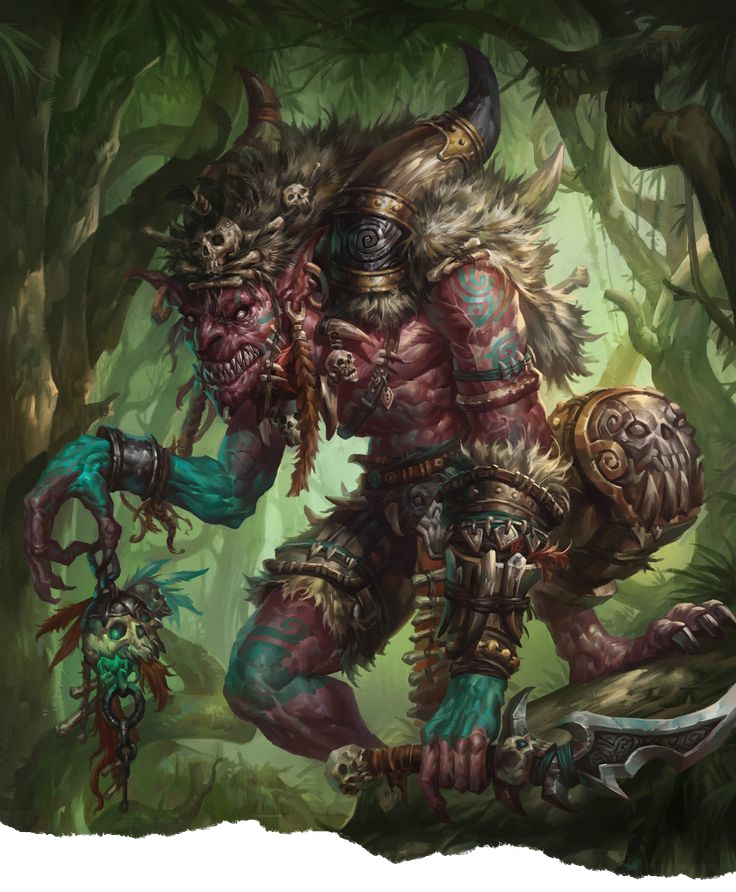
\includegraphics[scale=3.6]{media/chaman-hobgoblin.png}};
\end{tikzpicture}


% Monster stat block
\begin{DndMonster}[float*=b,width=\textwidth + 8pt]{Grommash Tejesombras}
    \begin{multicols}{2}
        \DndMonsterType{Chamán hobgoblin, caótico malvado}

    % If you want to use commas in the key values, enclose the values in braces.
    \DndMonsterBasics[
	armor-class = {12 con \emph{armadura de cuero}},
        hit-points  = {\DndDice{3d8 + 3}},
        speed       = {30 ft},
      ]

    \DndMonsterAbilityScores[
        str = 13,
        dex = 14,
        con = 13,
        int = 10,
        wis = 10,
        cha = 8,
      ]

    \DndMonsterDetails[
        %saving-throws = {Str +0, Dex +0, Con +0, Int +0, Wis +0, Cha +0},
        %skills = {Acrobatics +0, Animal Handling +0, Arcana +0, Athletics +0, Deception +0, History +0, Insight +0, Intimidation +0, Investigation +0, Medicine +0, Nature +0, Perception +0, Performance +0, Persuasion +0, Religion +0, Sleight of Hand +0, Stealth +0, Survival +0},
        %damage-vulnerabilities = {cold},
        %damage-resistances = {bludgeoning, piercing, and slashing from nonmagical attacks},
        %damage-immunities = {poison},
        %condition-immunities = {poisoned},
        senses = {visión en la oscuridad 120 pies, percepción pasiva 10},
        languages = {común, goblin, infernal},
        challenge = 3,
      ]
    % Traits
    \DndMonsterAction{Llamas infernales}
    Grommash puede lanzar llamas infernales en un área, causando daño de fuego a los enemigos cercanos.
    % \begin{DndMonsterSpells}
    %   \DndInnateSpellLevel{misty step}
    %   \DndInnateSpellLevel[3]{fog cloud, rope trick}
    %   \DndInnateSpellLevel[1]{identify}
    % \end{DndMonsterSpells}

    \DndMonsterAction{Teletransportación sombría}
    Puede usar una teletransportación sombría para moverse rápidamente a través de la oscuridad y aparecer en un 
    lugar diferente.

    \DndMonsterAction{Maleficio maldito}
    Maleficio Maldito: Puede lanzar un maleficio maldito sobre un objetivo, haciéndolo más vulnerable a los ataques.

    \DndMonsterSection{Acciones}
    \DndMonsterAction{Ataque con bastón mágico}
    Grommash puede usar su bastón mágico para lanzar rayos de energía a larga distancia o como arma de 
    combate cuerpo a cuerpo.

    \DndMonsterAction{Grito de guerra}
    Grommash emite un aterrador grito de guerra que inspira a sus seguidores goblins, dándoles un impulso 
    temporal en el combate.

    % %Default values are shown commented out
    % \DndMonsterAttack[
    %   name=Dagger,
    %   %distance=both, % valid options are in the set {both,melee,ranged},
    %   %type=weapon, %valid options are in the set {weapon,spell}
    %   mod=+3,
    %   %reach=5,
    %   %range=20/60,
    %   %targets=one target,
    %   dmg=\DndDice{1d4+1},
    %   dmg-type=piercing,
    %   %plus-dmg=,
    %   %plus-dmg-type=,
    %   %or-dmg=,
    %   %or-dmg-when=,
    %   %extra=,
    % ]

    % %\DndMonsterMelee calls \DndMonsterAttack with the melee option
    % \DndMonsterMelee[
    %   name=Flame Tongue Longsword,
    %   mod=+3,
    %   %reach=5,
    %   %targets=one target,
    %   dmg=\DndDice{1d8+1},
    %   dmg-type=slashing,
    %   plus-dmg=\DndDice{2d6},
    %   plus-dmg-type=fire,
    %   or-dmg=\DndDice{1d10+1},
    %   or-dmg-when=if used with two hands,
    %   %extra=,
    % ]

    % %\DndMonsterRanged calls \DndMonsterAttack with the ranged option
    % \DndMonsterRanged[
    %   name=Assassin's Light Crossbow,
    %   mod=+1,
    %   range=80/320,
    %   dmg=\DndDice{1d8},
    %   dmg-type=piercing,
    %   %plus-dmg=,
    %   %plus-dmg-type=,
    %   %or-dmg=,
    %   %or-dmg-when=,
    %   extra={, and the target must make a DC 15 Constitution saving throw, taking 24 (7d6) poison damage on a failed save, or half as much damage on a successful one}
    % ]

    \DndMonsterSection{Reacciones}
    \DndMonsterAction{Escudo arcano}
    Grommash puede reaccionar ante un ataque inminente creando un escudo arcano que reduce el daño recibido.

    \DndMonsterAction{Maldición vengativa}
    Si un enemigo le causa un daño significativo, Grommash puede lanzar una maldición vengativa sobre ese enemigo, 
    haciéndolo más vulnerable a futuros ataques.

    % Legendary Actions
    \DndMonsterSection{Acciones legendarias}
    Si Grommash logra completar el ritual de la luna de sangre, su poder se incrementa. Sus puntos de golpe y su CA se 
    multiplican por 10. Si logra sacrificar alguna de las niñas sus puntos de golpe y CA se multiplican por 2. Si sacrifica uno
    de los goblins en el foso de los sacrificios recupera la mitad de sus puntos de golpe y CA. En todo caso, realizar el 
    ritual de forma completa o parcial le permite lanzar una poderosa acción legendaria llamada ``Apoteosis de Sangre''. 
    Cuando activa esta acción, el cielo se oscurece totalmente y la tierra tiembla mientras canaliza la energía de la luna 
    de sangre.

    \begin{DndMonsterLegendaryActions}
      \DndMonsterLegendaryAction{Ataque devastador}{Grommash puede realizar un ataque devastador de área que inflige daño a todos los objetivos en un radio de 30 pies alrededor de él. Este ataque es una explosión de energía mágica en forma de una llamarada de fuego infernal.}
      \DndMonsterLegendaryAction{Parálisis temporal}{Todos los objetivos afectados por esta acción deben hacer una tirada de salvación contra una maldición que produce una parálisis temporal debido a la abrumadora presencia de Grommash.}
    \end{DndMonsterLegendaryActions}
  \end{multicols}
\end{DndMonster}


\chapter*{Sombrafauces}
\addcontentsline{toc}{section}{Sombrafauces}


\begin{tikzpicture}[remember picture, overlay]
    \node[anchor=north west] at ([xshift=-0.5cm,yshift=0.5cm]current page.north west){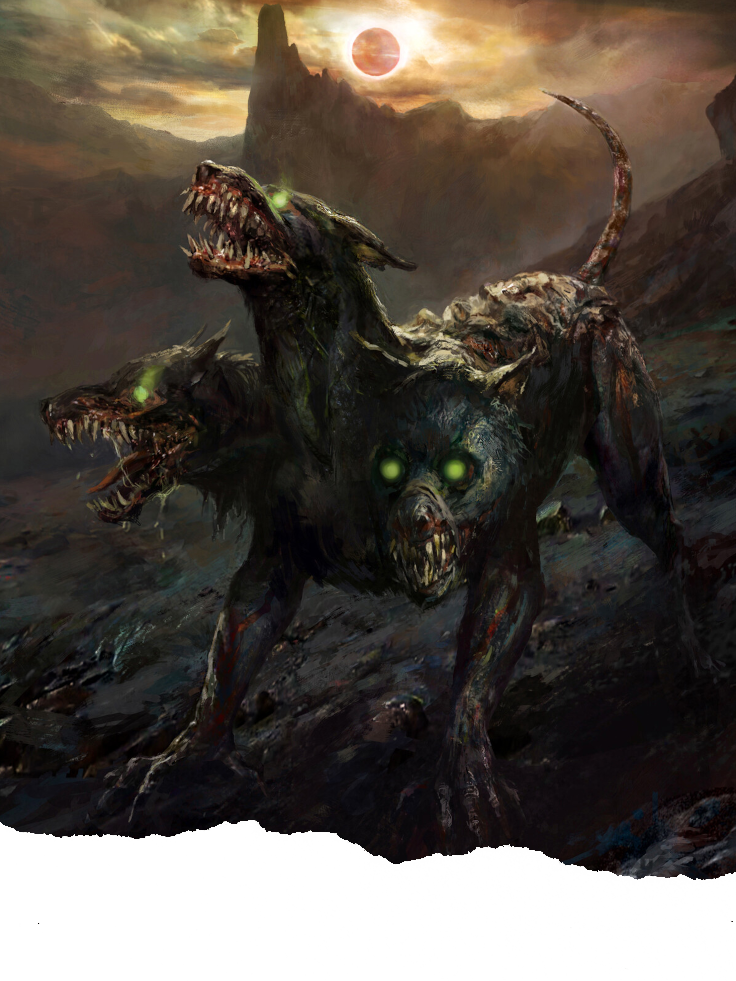
\includegraphics[scale=3.6]{media/hell-dog.png}};
\end{tikzpicture}


% Monster stat block
\begin{DndMonster}[float*=b,width=\textwidth + 8pt]{Sombrafauces - perro del inframundo}
    \begin{multicols}{2}
        \DndMonsterType{Monstruosidad mediana, caótico malvado}

    % If you want to use commas in the key values, enclose the values in braces.
    \DndMonsterBasics[
        armor-class = {12},
        hit-points  = {\DndDice{6d8 + 12}},
        speed       = {40 ft},
      ]

    \DndMonsterAbilityScores[
        str = 15,
        dex = 14,
        con = 14,
        int = 3,
        wis = 13,
        cha = 6,
      ]

    \DndMonsterDetails[
        %saving-throws = {Str +0, Dex +0, Con +0, Int +0, Wis +0, Cha +0},
        %skills = {Acrobatics +0, Animal Handling +0, Arcana +0, Athletics +0, Deception +0, History +0, Insight +0, Intimidation +0, Investigation +0, Medicine +0, Nature +0, Perception +0, Performance +0, Persuasion +0, Religion +0, Sleight of Hand +0, Stealth +0, Survival +0},
        %damage-vulnerabilities = {cold},
        %damage-resistances = {bludgeoning, piercing, and slashing from nonmagical attacks},
        %damage-immunities = {poison},
        %condition-immunities = {poisoned},
        senses = {visión en la oscuridad 120 pies, percepción pasiva 15},
        languages = {entiende infernal, pero no lo habla},
        challenge = 3,
      ]
    % Traits
    \DndMonsterAction{Teletransportación sombría}
    Puede ser teletransportado junto a Grommash Tejesombras a través de la oscuridad.

    \DndMonsterAction{Tres cabezas}
    El perro tiene ventaja en las pruebas de Sabiduría (Percepción) y en las tiradas de salvación para evitar ser
    asustado, aturdido, cegado, ensordecido, hechizado o dejado inconsciente.

    \DndMonsterSection{Acciones}
    \DndMonsterAction{Ataque múltiple}
    El perro realiza tres ataques de mordisco.

    %Default values are shown commented out
    \DndMonsterAttack[
      name=Mordisco,
      distance=melee, % valid options are in the set {both,melee,ranged},
      %type=weapon, %valid options are in the set {weapon,spell}
      mod=+4,
      reach=5,
      %range=20/60,
      targets=un objetivo,
      dmg=\DndDice{1d6+2},
      dmg-type=perforante,
      %plus-dmg=,
      %plus-dmg-type=,
      %or-dmg=,
      %or-dmg-when=,
      extra={. Si el objetivo es una criatura, debe superar una tirada de salvación de Constitución CD 12 contra enfermedad para no quedar envenenado hasta que se cure la enfermedad. Cada 24 horas, la criatura debe repetir la tirada de salvación y, si falla, su máximo de puntos de golpe se reduce en 5 (1d10). Esta reducción dura hasta que se cure la enfermedad. La criatura muere si la enfermedad reduce su máximo de puntos de golpe a 0},
    ]
  

  \end{multicols}
\end{DndMonster}

%%
%% Herramientas de ayuda
%%
\part*{Herramientas de ayuda}
%%
%%
%%

\chapter*{Herramientas de ayuda}
\addcontentsline{toc}{section}{Herramientas de ayuda}

\section*{Agarrar}
Cuando quieras agarrar o forcejees con una criatura tendrás que usar tu acción de Atacar para 
hacer un tipo especial de ataque cuerpo a cuerpo; agarrar. Si puedes realizar varios ataques 
con la acción de Atacar, este reemplaza a uno de ellos.

El objetivo de tu agarre debe estar dentro de tu alcance y tener un tamaño que esté como mucho 
una categoría por encima de la tuya. Utilizando al menos una mano libre, intentas sujetar al 
objetivo mediante una prueba de agarrar en lugar de una tirada de ataque: haz una prueba de 
Fuerza (Atletismo) enfrentada a una prueba de Fuerza (Atletismo) o Destreza (Acrobacias) del 
objetivo según elija este último.

Si tienes éxito, sometes a la víctima al estado \emph{agarrado}. Puedes liberar al objetivo 
cuando quieras, sin necesidad de invertir una acción. 

\textbf{Escapar de un agarre} . Una criatura agarrada puede utilizar su acción para intentar 
escapar. Lo logrará si tiene éxito en una prueba de Fuerza (Atletismo) o Destreza (Acrobacias) 
enfrentada a una prueba de Fuerza (Atletismo) de quien la tiene agarrada.

\textbf{Mover una criatura agarrada}. Cuando te muevas puedes arrastrar o transportar a la 
criatura agarrada, pero tu velocidad se reducirá a la mitad salvo si dicha criatura está dos o 
más categorías de tamaño por debajo de la tuya.

\textbf{Agarrar con una cuerda}. Realizar el agarre con una cuerda a distancia requiere una 
prueba de Destreza (Acrobacias) en lugar de la prueba de Fuerza (Atletismo). La cuerda debe 
tener una longitud igual o mayor a la distancia al objetivo y puedes añadir desventaja en la 
tirada si consideras que el jugador se encuentra demasiado lejos del objetivo. Por ejemplo, 
a más de 20 pies. Las cuerdas tienen 2 puntos de daño y se pueden romper si se les ataca o con 
una prueba de Fuerza CD 17.

\textbf{Fijar una cuerda}. Fijar una cuerda que tiene agarrada a una criatura requiere una 
acción. Haz una tirada de Destreza (Juego de manos) o Fuerza (Atletismo) para determinar 
la dificultad del agarre de la cuerda. La criatura agarrada podrá intentar escapar de ese 
agarre mediante una prueba de Fuerza (Athletismo) o Destreza (Acrobacias) enfrentada a esa 
dificultad calculada en el momento en que la cuerda se fijó.

\section*{Estados}

\subsection*{Agarrado}
\begin{itemize}
  \item La velocidad de una criatura agarrada es 0 y no puede aumentar por encima de ese valor.
  \item Este estado termina si quien agarra queda incapacitado.
  \item Este estado también termina si algún efecto aleja a la criatura de quien (o lo que) la 
  tiene agarrada, como cuando el conjuro ola atronadora hace salir despedida a una criatura.
\end{itemize}

\subsection*{Asustado}
\begin{itemize}
  \item Una criatura asustada tiene desventaja en las pruebas de característica y tiradas de 
  ataque mientras pueda ver a la fuente de su miedo.
  \item La criatura no puede acercarse a la fuente de su miedo voluntariamente.
\end{itemize}

\subsection*{Derribado}
\begin{itemize}
  \item Una criatura derribada solo podrá moverse arrastrándose, a no ser que se levante, 
  terminando así el estado.
  \item La criatura tiene desventaja en las tiradas de ataque.
  \item Las tiradas de ataque contra la criatura tienen ventaja si el atacante está a 5 pies o 
  menos de ella. Sin embargo, tienen desventaja si el atacante está a más distancia.
\end{itemize}

\subsection*{Envenenado}
\begin{itemize}
  \item Una criatura envenenada tiene desventaja en las tiradas de ataque y las pruebas de característica.
\end{itemize}

\subsection*{Incapacitado}
\begin{itemize}
  \item Una criatura incapacitada no puede llevar a cabo acciones ni reacciones.
\end{itemize}


%%
%% Página para contraportada
%%

% hack para que contraportada se muestre en página siguiente
\newpage
\mbox{}

% hack para crear la página vacía
\newpage
\thispagestyle{empty}
\mbox{}

% imagen de contraportada
\begin{figure}
  \begin{tikzpicture}[remember picture,overlay]
    \begin{scope}
    \node [xshift=0cm,yshift=0cm] at (current page.center){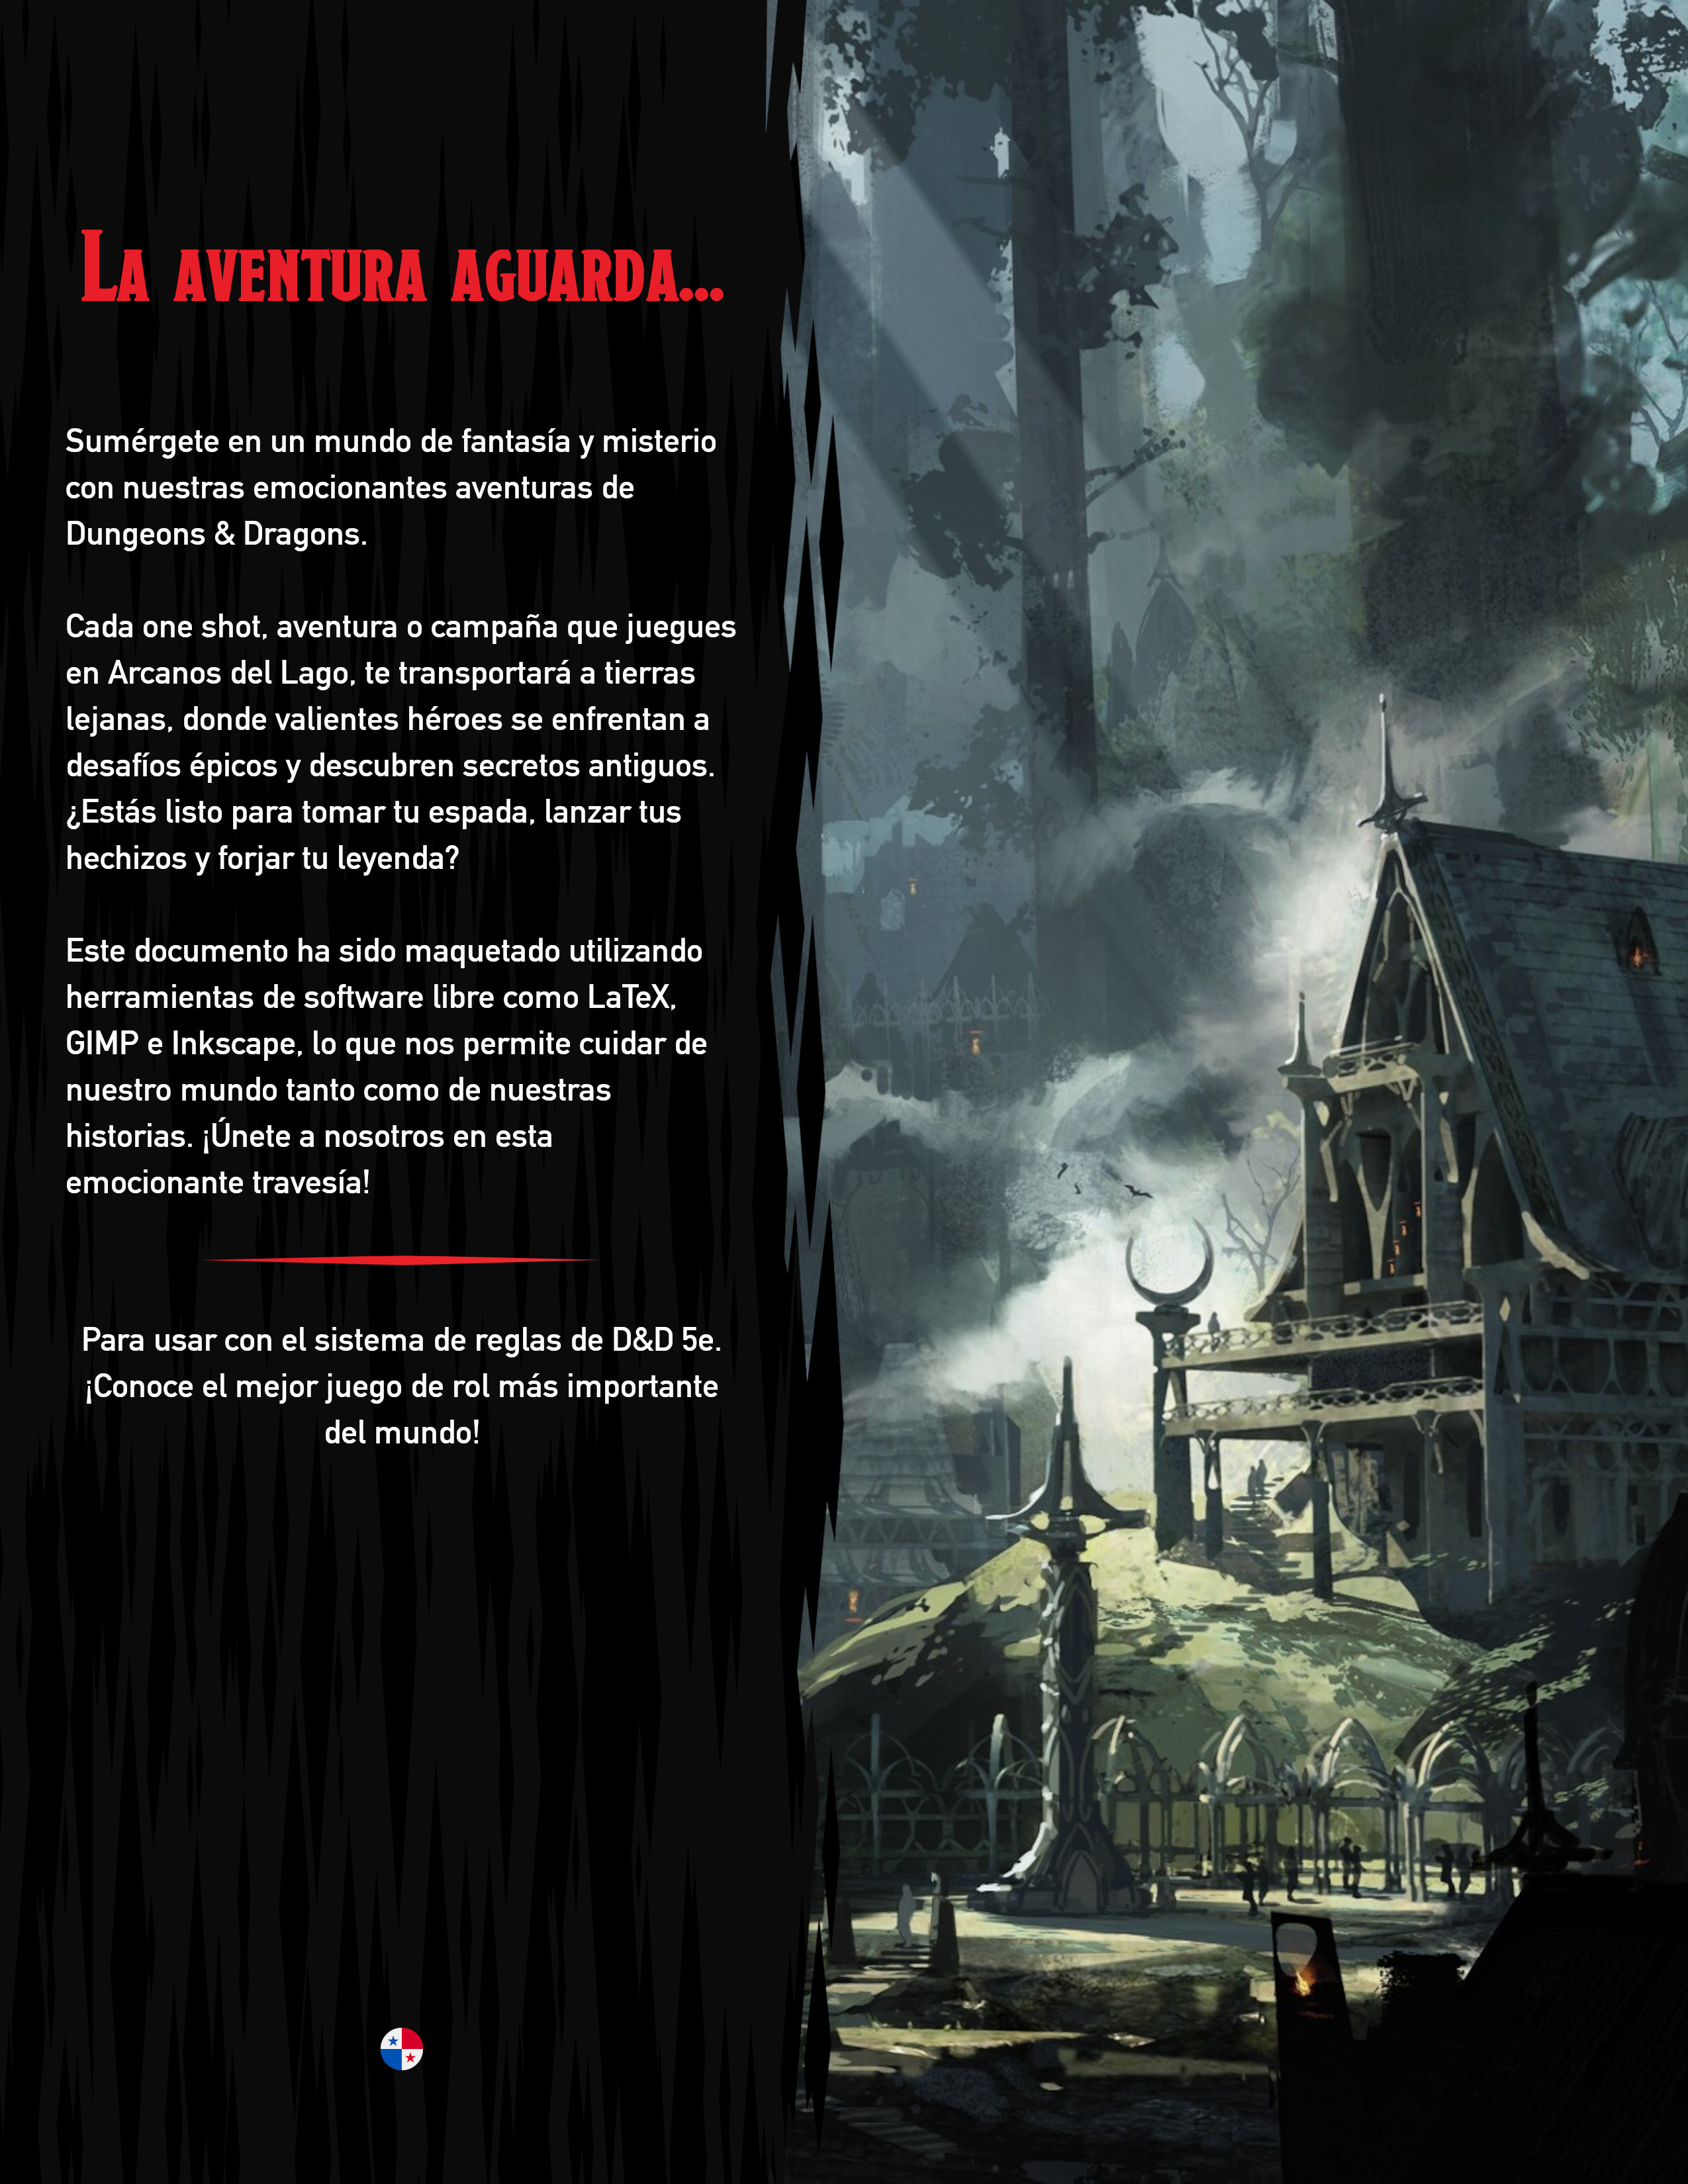
\includegraphics[width=\paperwidth]{covers/contraportada.jpg}};
    \end{scope}
  \end{tikzpicture}
\end{figure}

\end{document}